% =====================================================================
\section{Introduction}\label{sec:intro}
% =====================================================================

\subsection{Can one model have an uncomputable phase diagram?}

A classical lattice model assigns a finite set of local states to each site of $\Z^d$ and an energy to local patterns. Its equilibrium states at inverse temperature $\beta$ are its Gibbs measures, and its phase diagram records the values of $\beta$ at which the Gibbs measure is unique and those at which several phases coexist. For the two-dimensional Ising model the diagram is a single threshold, which Onsager computed exactly \cite{Onsager44}. Can the phase diagram of one fixed model, with a finite description, be impossible to compute?

For quantum spin systems at zero temperature the answer is yes. Cubitt, Perez-Garcia and Wolf proved that the spectral gap of translation-invariant nearest-neighbour Hamiltonians on a two-dimensional lattice is undecidable \cite{CPGW15,CPGW22}, and the same holds in one dimension \cite{BCLPG20}. Bausch, Cubitt and Watson then built one continuous family of such Hamiltonians $H(\varphi)$ whose phase cannot be computed from $\varphi$: on an interval of $\varphi$ starting at $2^{-n}$, the Hamiltonian is gapless with a critical ground state if a Turing machine halts on $n$, and gapped with a unique product ground state if it does not \cite{BCW21}. For classical models, Gu, Weedbrook, Perales and Nielsen showed that ground-state observables of two-dimensional Ising lattices built from Turing machines are undecidable, and expected the result to extend to positive temperature: it ``readily generalizes to lattices of finite temperatures'' \cite{GWPN09}. Gayral, Sablik and Taati wrote: ``We expect that, in two or more dimensions, most questions regarding the thermodynamic behaviour of finite-range models at or near zero temperature are undecidable'' \cite{GST25}.

This paper gives one fixed classical model, at positive temperature, whose phase diagram encodes the halting problem. It is a classical, positive-temperature counterpart of the quantum results above, with the temperature in the role of the parameter $\varphi$. The model has hard constraints: some local patterns have energy $+\infty$ and never occur.

\begin{mainA}[\cref{thm:main}]
Fix a universal Turing machine $U$. There are a finite set $\mathfrak S$ and a translation-invariant nearest-neighbour interaction $\Phi$ on $\mathfrak S^{\Z^2}$, with every local energy in $\{0,1,+\infty\}$ and with $U$ hard-coded, such that the following holds. Put $\lambda_K=2\sum_{j=0}^{K-1}\frac{1}{(2j+1)3^{2j+1}}$, $\beta_n=n\lambda_{n+3}$ and $J_n=(\beta_n-\frac1{1000},\beta_n+\frac1{1000})$ for $n\ge1$; these are pairwise disjoint intervals of positive numbers with rational endpoints computable from $n$. For every $n\ge1$ and every real $\beta\in J_n$:
\begin{enumerate}[label=\textup{(\roman*)}]
\item if $U$ does not halt on input $n$, then $\beta\Phi$ has exactly one translation-invariant Gibbs measure;
\item if $U$ halts on input $n$, then $\beta\Phi$ has at least two translation-invariant Gibbs measures.
\end{enumerate}
At every $\beta>0$, $\beta\Phi$ also has Gibbs measures that are not translation invariant: uniqueness in~(i) is uniqueness among translation-invariant Gibbs measures, and uniqueness among all Gibbs measures fails at every $\beta$.
\end{mainA}

Gibbs measures are taken with the standard convention for hard constraints: they are supported on the configurations of finite energy, and their conditional laws are Boltzmann weights over the admissible fillings of finite volumes (\cref{set:def-gibbs}). The partial sums $\lambda_K$ of the series $\log2=2\sum_{j\ge0}\frac{1}{(2j+1)3^{2j+1}}$ make $\beta_n$ rational and place it within $3/26244$ of $n\log 2$ (\cref{prf:windows}).

\begin{mainB}[\cref{cor:undecidable}]
The set of rational $\beta>0$ at which $\beta\Phi$ has exactly one translation-invariant Gibbs measure is undecidable: the rational number $\beta_n$, computable from $n$, belongs to it if and only if $U$ does not halt on $n$.
\end{mainB}

With the exact solution of the two-dimensional Ising model as an additional input, the whole diagram can be described: the coexistence set is a union of explicit intervals around $n\log2$, one for each $n$ on which $U$ halts (\cref{prop:exact}).

\subsection{How it works}

The interaction has two layers, drawn in \cref{fig:overview}. The \emph{background} is frozen by the hard constraints. The \emph{payload} carries Ising spins and fluctuates at temperature $\beta$.

\begin{itemize}
\item \emph{A frozen hierarchical tiling.} The bottom of the background is Ollinger's $2\times2$ substitution tiling \cite{Ollinger08}, in the transcription of \cite{LeanWang}, decorated with ruler bits \cite{DM26forget}. It has exactly one translation-invariant probability measure, and almost every tiling under it is rigid: no change of finitely many tiles gives another tiling (\cref{prop:scaffold-ti}).
\item \emph{Grids at every depth.} The light red squares of the tiling are nested frames. Following Robinson's method \cite{Robinson71}, the frames of depth $d$ cut out square grids of $N_d\times N_d$ sites, $N_d=2^{d+2}-2$, joined by straight channels (\cref{prop:routing}). Every depth occurs with positive density.
\item \emph{A computation on each grid.} A static binary counter on each grid finds $d$. A fixed Turing machine $M$ computes the \emph{label} $n(d)=1+v_2(d)$, where $v_2$ is the $2$-adic valuation, and runs $U$ on $n(d)$ inside the grid. The grid is \emph{ready} if this computation halts before the grid ends (\cref{bg:ready}). Every label is the label of infinitely many depths, so if $U$ halts on $n$, every sufficiently large depth with label $n$ is ready.
\item \emph{Ising layers from sensors.} Every site carries a free spin. Wires join the spin at the south-west corner, the \emph{root}, of each grid to the roots of the next grids of the same depth. At a ready root two \emph{sensors} compare the root spin with the incoming wires. A sensor is a finite gadget of free bits and unit energies; summing over it gives exactly an Ising coupling $J_n(\beta)$ between neighbouring roots, with $e^{2J_n}=1+1/b_n$ and
\[
b_n(\beta)=2^{-4}\cosh\bigl(20(\beta-n\log2)\bigr)+2^{-10}
\]
(\cref{pay:sum}). The coupling is strong ($e^{J_n}>3$) when $|\beta/\log2-n|<1/20$ and very weak at distance at least $19/20$.
\end{itemize}

So for $\beta\in J_n$ the payload is a disjoint union of Ising models, one for each ready depth. All of them are in the high-temperature regime of Dobrushin's uniqueness theorem unless some ready depth has label $n$, which happens exactly when $U$ halts on $n$; then the Peierls argument gives two phases. Integrating the payload over the frozen background turns these statements into statements about translation-invariant Gibbs measures of $\beta\Phi$ (\cref{sec:proof}).

\begin{figure}[ht]
\centering
\resizebox{\textwidth}{!}{%
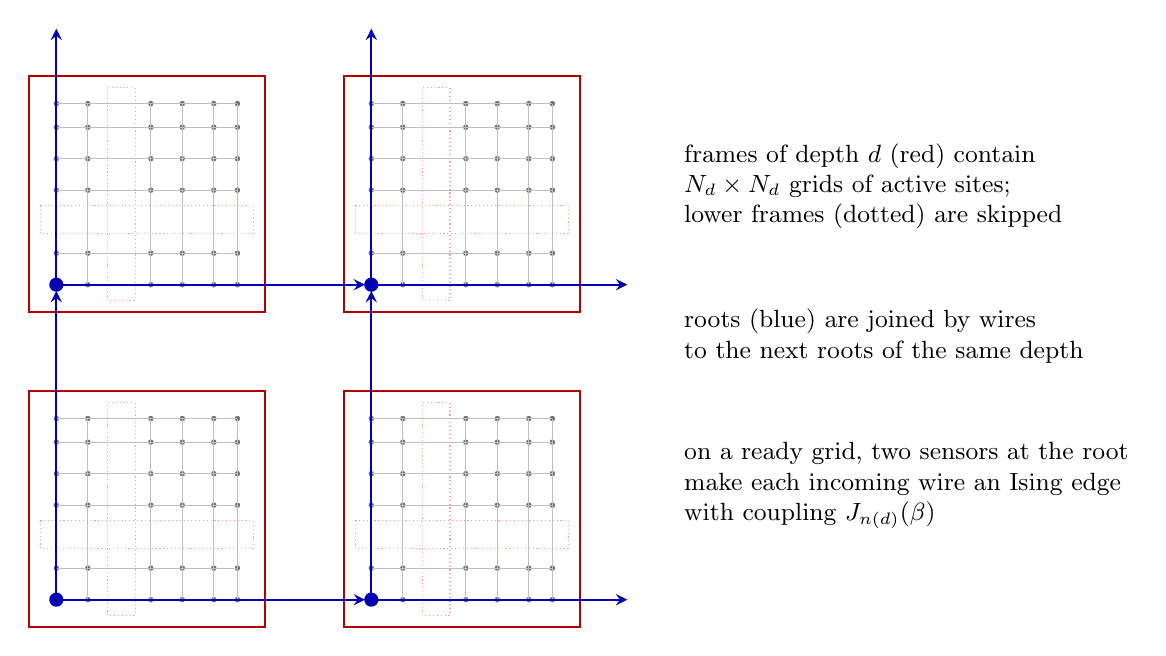
\begin{tikzpicture}[>=stealth,font=\small]
\foreach \X in {0,4}{\foreach \Y in {0,4}{
 \draw[red!70!black,thick] (\X,\Y) rectangle (\X+3,\Y+3);
 \foreach \i in {0.35,0.75,1.55,1.95,2.35,2.65}{\foreach \j in {0.35,0.75,1.55,1.95,2.35,2.65}{\fill[black!55] (\X+\i,\Y+\j) circle (0.035);}}
 \foreach \i in {0.35,0.75,1.55,1.95,2.35,2.65}{\draw[black!25] (\X+\i,\Y+0.35)--(\X+\i,\Y+2.65); \draw[black!25] (\X+0.35,\Y+\i)--(\X+2.65,\Y+\i);}
 \draw[red!40,densely dotted] (\X+1.0,\Y+0.15) rectangle (\X+1.35,\Y+2.85);
 \draw[red!40,densely dotted] (\X+0.15,\Y+1.0) rectangle (\X+2.85,\Y+1.35);
 \fill[blue!70!black] (\X+0.35,\Y+0.35) circle (0.09);
}}
\draw[blue!70!black,thick,->] (0.35,0.35)--(4.27,0.35);
\draw[blue!70!black,thick,->] (0.35,4.35)--(4.27,4.35);
\draw[blue!70!black,thick,->] (0.35,0.35)--(0.35,4.27);
\draw[blue!70!black,thick,->] (4.35,0.35)--(4.35,4.27);
\draw[blue!70!black,thick,->] (4.35,4.35)--(7.6,4.35);
\draw[blue!70!black,thick,->] (4.35,4.35)--(4.35,7.6);
\draw[blue!70!black,thick,->] (0.35,4.35)--(0.35,7.6);
\draw[blue!70!black,thick,->] (4.35,0.35)--(7.6,0.35);
\node[anchor=west,align=left] at (8.2,5.6) {frames of depth $d$ (red) contain\\ $N_d\times N_d$ grids of active sites;\\ lower frames (dotted) are skipped};
\node[anchor=west,align=left] at (8.2,3.7) {roots (blue) are joined by wires\\ to the next roots of the same depth};
\node[anchor=west,align=left] at (8.2,1.8) {on a ready grid, two sensors at the root\\ make each incoming wire an Ising edge\\ with coupling $J_{n(d)}(\beta)$};
\end{tikzpicture}}
\caption{The two layers of the model, schematically. Inside each frame of depth $d$, the sites whose row and column avoid all lower frames form an $N_d\times N_d$ grid, on which the machine $M$ runs. The roots of all grids of depth $d$ form a square lattice of spacing $4^{d+1}$. Each root sends its spin east and north along wires; when the grids of depth $d$ are ready, sensors at the receiving roots turn these wires into the edges of an Ising model with coupling $J_{n(d)}(\beta)$.}
\label{fig:overview}
\end{figure}

\subsection{Objections answered}

\paragraph{The hard constraints.} The model is a hard-constraint model, and the infinite energies are essential to the proof. They freeze the background, so that finite-volume conditional laws cannot change the tiling, the grids or the computations, and they keep every computation exact. Nothing in this paper applies to interactions with finite energies only. For finite-range interactions with computable finite energies, the pressure is a computable function of $\beta$ when the configuration space is a full shift \cite[Proposition~14]{GST25}. A finite-energy version of Theorem~A is the first open problem of \cref{sec:open}.

\paragraph{Translation invariance.} Each typical frozen background, with the payload in equilibrium on it, is a Gibbs measure that is not translation invariant. So at every $\beta$ there are uncountably many Gibbs measures, and the statement about uniqueness concerns the translation-invariant ones; Theorem~A states this. In case~(i), the unique translation-invariant Gibbs measure is the average of the payload equilibria over the unique translation-invariant law of the background.

\paragraph{Is the input hidden in the interaction?} No. The interaction is one finite table, fixed before $n$. The intervals $J_n$ are computable from $n$ without knowing whether $U$ halts. The halting of $U$ on $n$ enters only through which grids of the frozen background complete their computation.

\paragraph{Probabilistic cellular automata.} Kurdyumov \cite{Kurdyumov78} and Toom \cite{Toom00} proved that ergodicity of probabilistic cellular automata is undecidable, for automata in which some transitions have probability zero; see also \cite{BMM13}. The space--time histories of such an automaton form a lattice system one dimension up with hard constraints, so these results already concern classes of hard-constraint systems, with one system for each machine. In \cite{DM26forget} we showed that ergodicity remains undecidable for a computable family of automata with positive rates, all at one fixed noise rate, and deduced that uniqueness of the translation-invariant Gibbs measure is undecidable for the associated family of space--time interactions; there too the machine is part of the model. Here the interaction is fixed and the input is carried by the temperature.

\subsection{Prior work}

\Cref{tab:landscape} places Theorem~A among the closest results. In \cite{DM26thermal} we proved that, at one fixed positive temperature, spontaneous magnetization, exponential decay of a specified spin correlation and uniqueness of the Gibbs measure are undecidable for computable families of translation-invariant finite-range interactions on $\Z^2$ with strictly positive rational Boltzmann weights; there the input is a cellular automaton from a family with undecidable surjectivity, and the interaction, including its range, depends on it. Theorem~A instead fixes one nearest-neighbour interaction, with hard constraints, lets the input enter only through the inverse temperature, and makes undecidable uniqueness among translation-invariant Gibbs measures, not among all Gibbs measures. Mi\k{e}kisz and Taati built a finite-range lattice gas on $\Z^4$ whose low-temperature Gibbs states are perturbations of Ammann tilings, by running a noise-resilient computation inside its Gibbs states \cite{TaatiMiekisz26}. Computability also enters thermodynamics through zero-temperature limits of Gibbs measures \cite{ChazottesHochman10} and through the entropies of multidimensional subshifts of finite type \cite{HochmanMeyerovitch10}. Marsan, Sablik and T\"orm\"a built a perturbed cellular automaton whose ergodicity undergoes at least two transitions as the noise varies, and asked which sets of noise parameters can occur as ergodicity sets \cite{MarsanSablikTorma26}. The scaffold uses Wang tiles \cite{Wang61}, the hierarchical method of Berger \cite{Berger66} and Robinson \cite{Robinson71}, and substitution tilings with local rules and unique derivation \cite{Mozes89,Mosse92,Solomyak98}, through Ollinger's substitution \cite{Ollinger08} as transcribed in \cite{LeanWang}; the ruler decoration and its proofs are from \cite{DM26forget}.

\begin{table}[ht]
\centering
\small
\begin{tabularx}{\textwidth}{@{}>{\raggedright\arraybackslash}X>{\raggedright\arraybackslash}p{2.1cm}>{\raggedright\arraybackslash}p{2.3cm}>{\raggedright\arraybackslash}p{2.6cm}>{\raggedright\arraybackslash}p{2.0cm}@{}}
\toprule
Result & System & Temperature & One fixed model & Local terms\\
\midrule
Undecidable spectral gap \cite{CPGW15,CPGW22} & quantum & zero & no & finite\\
Uncomputable phase diagram \cite{BCW21} & quantum & zero & yes, parameter $\varphi$ & finite\\
Undecidable ergodicity of automata \cite{Kurdyumov78,Toom00} & classical & dynamics & no & some zero\\
Undecidable ground-state observables \cite{GWPN09} & classical & zero & no & finite\\
Undecidable chaoticity \cite{GST25} & classical & zero (limit) & no & finite\\
Undecidable magnetization and uniqueness \cite{DM26thermal} & classical & positive & no & finite\\
Undecidable ergodicity at fixed noise \cite{DM26forget} & classical & positive & no & finite\\
Theorem~A & classical & positive, parameter $\beta$ & yes & $\{0,1,+\infty\}$\\
\bottomrule
\end{tabularx}
\caption{Undecidability of phases. ``One fixed model'' means that the interaction is fixed and the input enters only through a real parameter. ``Some zero'' means that some transition probabilities vanish; for \cite{DM26forget} the local weights are the positive transition probabilities of the automata.}
\label{tab:landscape}
\end{table}

\subsection{Reading guide}

\Cref{sec:setting} fixes the definitions: interactions with hard constraints, Gibbs measures, Turing machines, and two classical facts about the Ising model. \Cref{sec:scaffold} presents the scaffold and proves that it has one translation-invariant law and is rigid; the finite-table proofs about the substitution are in \cref{app:scaffold}. \Cref{sec:interaction} defines the interaction completely: every field, every local constraint and every energy term. Its tables are collected in \cref{app:tables}, and the machine $M$ is given in \cref{app:machine}. \Cref{sec:background} shows that the background is determined by the scaffold and computes it. \Cref{sec:payload} eliminates the sensors and identifies the payload with a disjoint union of Ising models. \Cref{sec:proof} proves Theorem~A and Corollary~B. \Cref{sec:exact} gives the exact diagram, conditional on the classical solution of the Ising model, and \cref{sec:open} lists open problems. A reader interested only in the thermodynamics can take \cref{prop:background,lem:freeze} and \cref{pay:effective} as black boxes and read \cref{sec:proof}.
